
%%%%%%%%%%%%%%%%%%%%%%%%%%%%%%%%%%%%%%%%%%%%%%%%%%%%%%%%%%%%%%%%%%%%
% 이 파일에는 본문 내용을 입력하면 된다.
%%%%%%%%%%%%%%%%%%%%%%%%%%%%%%%%%%%%%%%%%%%%%%%%%%%%%%%%%%%%%%%%%%%%


\section{서론} % 섹션을 시작할 때는  \section{섹션제목} 와 같은 형태로 섹션 제목을 쓰고 그 아래에 본문을 쓰면 된다.

\jiwon[2] % 더미 텍스트

\section{이론적 배경 및 선행연구 조사}\label{sec:search}
\subsection{소제목}
\subsubsection{과학영재 창의연구(R\&E)}

\jiwon[6-7] % 더미 텍스트

앞서 \ref{sec:search}절에서 본 바와 같이 이론적 배경은 매우 어렵다.


\begin{figure}[!ht] % 그림입력
    \centering
    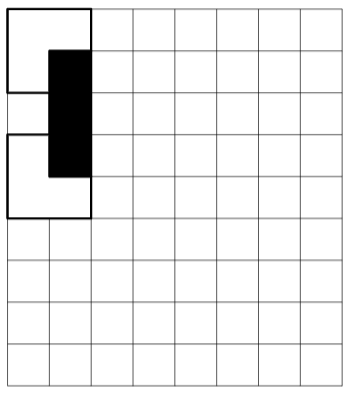
\includegraphics[width=.15\textwidth]{images/B(8, 9).png} % images/그림파일 이름
    \caption{bad pair of $9\times 8$ deficient tile} % 그림 캡션
    \label{fig:my_label} % 그림의 위치를 지시할 때 쓰는 label
\end{figure}

\begin{definition}
정의란 무엇일까? \citep{aanjaneya2009tromino, golomb2021polyominoes, nitica2017tilings} % 참고문헌 표기
\end{definition}

\jiwon[3-4] % 더미 텍스트

\begin{theorem}\label{thm:what}
    정리란 무엇일까?
\end{theorem}



\subsection{그림 삽입 방법}

%--------- 그림 삽입 방법 설명(내용을 확인 한 후에, 삭제하세요).
아래에서는 그림을 삽입하는 방법을 안내한다. 크게 두 가지 방법이 있다.
\begin{enumerate}[(a)]
    \item 그림 파일을 images 폴더에 업로드 한 후, 그 파일을 넣는 방식.
    \item 텍을 이용하여 직접 그림을 그리는 방식.
\end{enumerate}
그러나, 어느 방식이든, 그림의 위치를 \TeX에게 맡기려면, figure 환경을 이용해야한다. 또 하나의 팁을 주자면, 그림파일을 미리 준비하지 않았더라도, \TeX이 갖고 있는 예시그림을 이용하여 그림의 위치를 미리 어느 정도 살펴볼 수 있다는 것이다. 

다음 예시는 \TeX이 갖고 있는 그림예제를 이용하여 그림을 삽입해 본 것이다.

\begin{figure}[!ht]
    \centering
    \includegraphics[width=.4\textwidth]{example-image} % images/그림파일 이름
    \caption{이 그림의 캡션은?!}
    \label{fig:my_fig_label}
\end{figure}


다음 예시는 텍을 이용하여 직접 그림을 그리는 예이다.
\begin{center}
 \begin{tikzpicture}[scale=.5]
 	\checkerboard{15}{15} 	% 그리드를 그리는 명령 \checkerboard{"가로칸 수"}{"세로칸 수"}
	\LtrominoNE{3}{10}
	\LtrominoNW{4}{0}
	\LtrominoSW{6}{1}
	\LtrominoSE{10}{5}
 \end{tikzpicture}
\end{center}
이 그림은 figure 환경에 그린 것이 아니기 때문에, 별도의 캡션이 달려있지는 않다.  figure 환경에 넣은 그림에는 각 그림에 label을 지정해두었으므로, 상호참조 기능을 이용하여 ``그림 \ref{fig:my_label}\을 참고하라.''와 같이 해당 그림을 언급할 수 있다.

한가지 유의할 점은, 논문에서 그림은 필요한 경우에만 넣는 다는 것이다. 다시 말해, 논문에 그림을 넣는 것은 논문의 내용에 (상호참조 등을 통해) 그 그림이 언급하만 가능한 것으로 여기는 것이 일반적이다. 따라서 논문에 등장하는 모든 그림은 figure 환경에 넣는 것이 바람직하다 하겠다.

%------------ 그림 삽입 방법 설명 끝. 

\subsection{표 삽입 방법}
한편 표를 삽입하는 방법은 그림을 삽입하는 방법과 거의 동일하다. figure 환경을 table환경으로 바꾸기만 하면 된다. 표를 텍에서 집접 그리는 것은 좀 번거로울 수 있다. 불편하다면, 다른 표 작성도구로 표를 만든 다음 이를 그림으로 집어 넣되 다만 table 환경을 이용하여 삽입하면 캡션이 자연스럽게 잘 붙을 것이다.

\begin{table}[!ht]
    \centering
    % 표를 만드는 가장 좋은 환경은 tblr 환경이다. (tabularray페키지 필요) 그리고 https://www.tablesgenerator.com/ 를 이용하면 아주 편리하다.
    \caption{이 표의 캡션은?!}
    \label{tab:my_label}
    \begin{tblr}{
    hlines,vlines
    }
          & 위치 & 장소 \\ 
        1 &    &    \\ 
        2 &    &    \\ 
        3 &    &    \\ 
    \end{tblr}
\end{table}

한편 표 \ref{tab:my_booktablabel}에서 볼 수 있는 표 양식은 여러 타이포그라피 교과서에서 권장하는 양식이며, 서구권에서 표준적으로 사용하는 양식이라 할 수 있다.
\begin{table}[!ht]
    \centering
    % 표를 만드는 가장 좋은 환경은 tblr 환경이다. (tabularray페키지 필요) 그리고 https://www.tablesgenerator.com/ 를 이용하면 아주 편리하다.
    \caption{예쁜 표의 캡션은?!}
    \label{tab:my_booktablabel}
\begin{booktabs}{
colspec={cccc}
}
\toprule
Case & Box A & Box B & Remarks \\
\midrule
\SetCell[r=2]{c,m} A & $+X$ & $-1.0$ & \SetCell[r=2]{c,m} B \\
\cmidrule[lr]{2-3}
& $-X$ & $-7.9$ & & \\
\bottomrule
\end{booktabs}
\end{table}


\subsection{수식 입력 방법}
이번에는 수식을 작성하는 몇 가지 예를 살펴보자. 수식은 크게 두 가지 모드로 작성한다.
\begin{itemize}
    \item 행중수식: 문단을 바꾸지 않고 쓰는 수식
    \item 행간수식: 문단을 별도로 두어 별도의 행에 쓰는 수식
\end{itemize}
구체적인 몇 가지 예를 통해서 수식을 입력하는 방법을 살펴보자.

%----------- 수식 작성 예졔
\begin{itemize}
    \item 아래첨자.

아래첨자는, 예를 들어, 이렇게 쓰면 된다. $A_{b+c}$. 여기서 $A_a+b$와 비교해보아라. 아! 그리고 곱하기는 $a\times b$와 같이 쓴다.
\item 최대정수함수 기호. 

국제표준(?) 방식으로 써보자. $\lfloor x\rfloor$로 쓰면 된다. 최대정수함수를 비롯한, 소위, 괄호류(?)는 괄호 안에 들어 있는 수식의 크기에 맞게 괄호의 크기가 바뀌어야겠죠! 아래의 두 식을 비교해 보세요.
\[ \lfloor \frac{\pi^2}{6}\rfloor \]
으, 못생긴 식이다.
\[ \left\lfloor \frac{\pi^2}{6}\right\rfloor \]
그렇다. $\left( \frac{1}{2} \right)$와 같이 쓰면 된다.

\item 분수 표기는 $\frac{2}{3}$과 같이 쓰면 된다. 행간수식을 이용해서 분수를 표기하면 
\[ \frac{df}{dt}=\frac{df}{ds}\frac{ds}{dt} \]
와 같이 분수의 크기가 커진다.


\item 부등호는 알다시피 $1\leq 3\leq 5 \geq 2$.

\item 합동식.

몇 가지 방법이 있다. 우선 세 줄짜리 등호는 $\equiv$ 이렇게. 아래에서는 여러 줄에 걸친 수식을 쓰는 법도 함께 보자. 소스에 등장하는 \& 는 수식을 정렬하는 도구로 이해하면 된다. 줄바꿈은 백슬래시 두 개!
\begin{align*}
a & \equiv b \mod{p} \\
a & \equiv b \pmod{p}
\end{align*}
음, 두 번째 방법으로 쓰면 되겠구나.
\end{itemize}
%---------- 수식 작성 예제 끝.



\section{결론} 
\jiwon[4] % 더미 텍스트



